% !TeX root = ../sn.tex
\documentclass[../sn.tex]{subfiles}

\begin{document}

\subsection{Introduction}
P4 is domain-specific programming language for network devices, specifying how data plane devices process packets.
It is vendor-agnostic and protocol-agnostic and it aims at making easier the implementation of software packets processing pipeline instead of waiting years to develop a new chip.
P4 is a declarative language, each P4 program follow the same workflow.
P4 programs and compilers are target-specific (FPGA, Programmable ASICs or software x86).

A P4 program classifies packets by header according to the definition provided by the programmer in the program.
As said before P4 is protocol-agnostic so you must declare every header you want to use because even the most common headers are not provided by the standard library.
The image below represents the working flow of a P4 program:
\begin{center}
    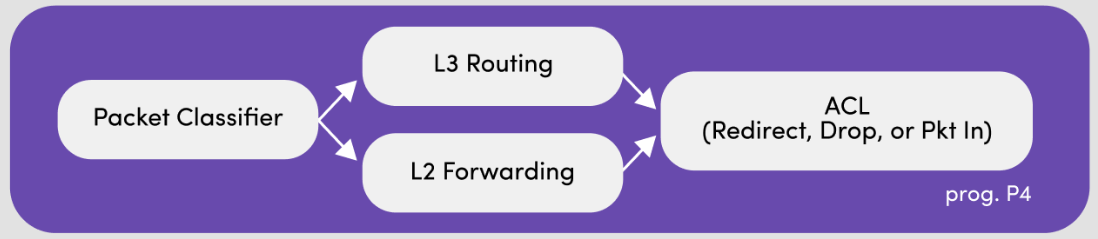
\includegraphics[scale=0.3]{p4_workflow.png}
\end{center}
The compiler produces an executable file for the given data plane target and a config file which allows the control and dataplane to communicate using P4Runtime.

P4 provides a single primitive type which is \emph{bit} and it is used to define headers like the following one:
\begin{lstlisting}
    typedef bit<48> macAddr_t;

    header ethernet_t {
        macAddr_t dstAddr;
        macAddr_t srcAddr;
        bit<16>   etherType
    }
\end{lstlisting}
In the source code a classifier is called \emph{Programmable Parser} and it is basically an ordered definition of headers which is used to matches the inbound packets and classifies them

\begin{lstlisting}

\end{lstlisting}
\end{document}